% mycsrf 'for beeing included' snippet template
%
% (c) Karsten Reincke, Frankfurt a.M. 2012, ff.
%
% This text is licensed under the Creative Commons Attribution 3.0 Germany
% License (http://creativecommons.org/licenses/by/3.0/de/): Feel free to share
% (to copy, distribute and transmit) or to remix (to adapt) it, if you respect
% how you must attribute the work in the manner specified by the author(s):
% \newline
% In an internet based reuse please link the reused parts to mycsrf.fodina.de
% and mention the original author Karsten Reincke in a suitable manner. In a
% paper-like reuse please insert a short hint to mycsrf.fodina.de and to the
% original author, Karsten Reincke, into your preface. For normal quotations
% please use the scientific standard to cite
%

\tikzstyle{nodv} = [font=\small, ellipse, draw, fill=gray!10, 
    text width=2cm, text centered, minimum height=2em]

\tikzstyle{nods} = [font=\footnotesize, rectangle, draw, fill=gray!20, 
    text width=1.2cm, text centered, rounded corners, minimum height=3em]

\tikzstyle{nodb} = [font=\footnotesize, rectangle, draw, fill=gray!20, 
    text width=2.2cm, text centered, rounded corners, minimum height=3em]

\tikzstyle{nodx} = [font=\footnotesize, rectangle, draw, fill=gray!20, 
    text width=2.4cm, text centered, rounded corners, minimum height=3em]
    
\tikzstyle{leaf} = [font=\tiny, rectangle, draw, fill=gray!30, 
    text width=1.2cm, text centered, minimum height=6em]

\tikzstyle{edge} = [draw, -latex']

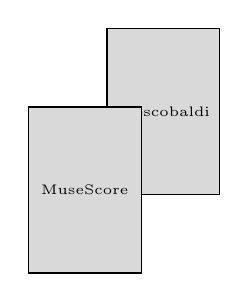
\begin{tikzpicture}[]

%\node (l61) at ( 2.4, 9.2) {MIT};

%\node[nodb] (l51) at ( 0.0, 7.8) {\textit{recipient:} \\ \textbf{4yourself}};
% \node[nodb] (l52) at ( 4.8, 7.8) {\textit{recipient:} \\ \textbf{2others}};
% 
% \node[nodb] (l41) at ( 2.5, 6.2) {\textit{state:} \\ \textbf{unmodified}};
% \node[nodb] (l42) at ( 7.0, 6.2) {\textit{state:} \\ \textbf{modified}};
% 
% \node[nodb] (l31) at ( 5.0, 4.6) {\textit{type:} \\ \textbf{proapse}};
% \node[nodb] (l32) at ( 9.0, 4.6) {\textit{type:} \\ \textbf{snimoli}};
% 
% \node[nodx] (l21) at ( 7.5, 2.8) {\textit{context:} \\ \textbf{independent}};
% \node[nodx] (l22) at (10.5, 2.8) {\textit{context:} \\ \textbf{embedded}};
% 
% \node[leaf] (l11) at ( 0.0, 0.0) {\textbf{MIT-C1} \textit{using software only for yourself}};
% \node[leaf] (l12) at ( 2.5, 0.0) {\textbf{MIT-C2} \textit{distributing unmodified package}};
% \node[leaf] (l13) at ( 5.0, 0.0) {\textbf{MIT-C3} \textit{distributing modified program}};
% \node[leaf] (l14) at ( 7.5, 0.0) {\textbf{MIT-C4} \textit{distributing modified library as independent package}};



\node[leaf] (l14) at (1.0cm, 1.0cm) {Frescobaldi};

\node[leaf] (l15) at (0.0, 0.0) {MuseScore};


% \path [edge] (l61) -- (l51);
% \path [edge] (l61) -- (l52);
% \path [edge] (l51) -- (l11);
% \path [edge] (l52) -- (l41);
% \path [edge] (l52) -- (l42);
% \path [edge] (l41) -- (l12);
% \path [edge] (l42) -- (l31);
% \path [edge] (l42) -- (l32);
% \path [edge] (l31) -- (l13);
% \path [edge] (l32) -- (l21);
% \path [edge] (l32) -- (l22);
% \path [edge] (l21) -- (l14);
% \path [edge] (l22) -- (l15);

\end{tikzpicture}





% this is only inserted to eject fault messages in texlipse
%\bibliography{../bib/literature}
